\documentclass[11pt]{article}
\usepackage{geometry}
\geometry{letterpaper}

\usepackage{graphicx}
% \usepackage[outdir=../img/]{epstopdf}
\usepackage{amssymb, amsmath}
\usepackage{epstopdf}
\usepackage[usenames,dvipsnames]{color}
\usepackage{listings}
\usepackage{pdfpages}
\usepackage{booktabs}
\usepackage[hyperref=auto,style=alphabetic,backend=bibtex]{biblatex}
\usepackage[colorlinks]{hyperref}
% \usepackage[numbered,framed]{matlab-prettifier}
\DeclareGraphicsRule{.tif}{png}{.png}{`convert #1 `dirname #1`/`basename #1 .tif`.png}
\addbibresource{report.bib}

\setlength{\parskip}{\baselineskip}     % space between paragraphs
\setlength{\parindent}{0pt}             % indenting of each paragraph

%\title{Title}
%\author{Name 1, Name 2}
%\date{date}

\begin{document}


%!TEX root = report.tex
\thispagestyle{empty}

\begin{center}
\includegraphics[width=5cm]{ETHlogo.eps}

\bigskip


\bigskip


\bigskip


\LARGE{ Lecture with Computer Exercises:\\ }
\LARGE{ Modelling and Simulating Social Systems with MATLAB\\}

\bigskip

\bigskip

\small{Project Report}\\

\bigskip

\bigskip

\bigskip

\bigskip


\begin{tabular}{|c|}
\hline
\\
\textbf{\LARGE{Traffic simulation in the city of Z\"urich}}\\
\\
\hline
\end{tabular}
\bigskip

\bigskip

\bigskip

\LARGE{Jan D\"{o}rrie, Simone Forte, \\Charalampos Gkonos, Athina Korfiati}



\bigskip

\bigskip

\bigskip

\bigskip

\bigskip

\bigskip

\bigskip

\bigskip

Z\"urich\\
May 2014\\

\end{center}



\newpage

%%%%%%%%%%%%%%%%%%%%%%%%%%%%%%%%%%%%%%%%%%%%%%%%%

% \newpage
% \section*{Agreement for free-download}
% \bigskip


% \bigskip


% \large We hereby agree to make our source code for this project freely available for download from the web pages of the SOMS chair.
% Furthermore, we assure that all source code is written by ourselves and is not violating any copyright restrictions.

% \begin{center}

% \bigskip


% \bigskip

% \vspace{2cm}

% Jan D\"{o}rrie \hfill Simone Forte \hfill Charalampos Gkonos \hfill Athina Korfiati

% \end{center}

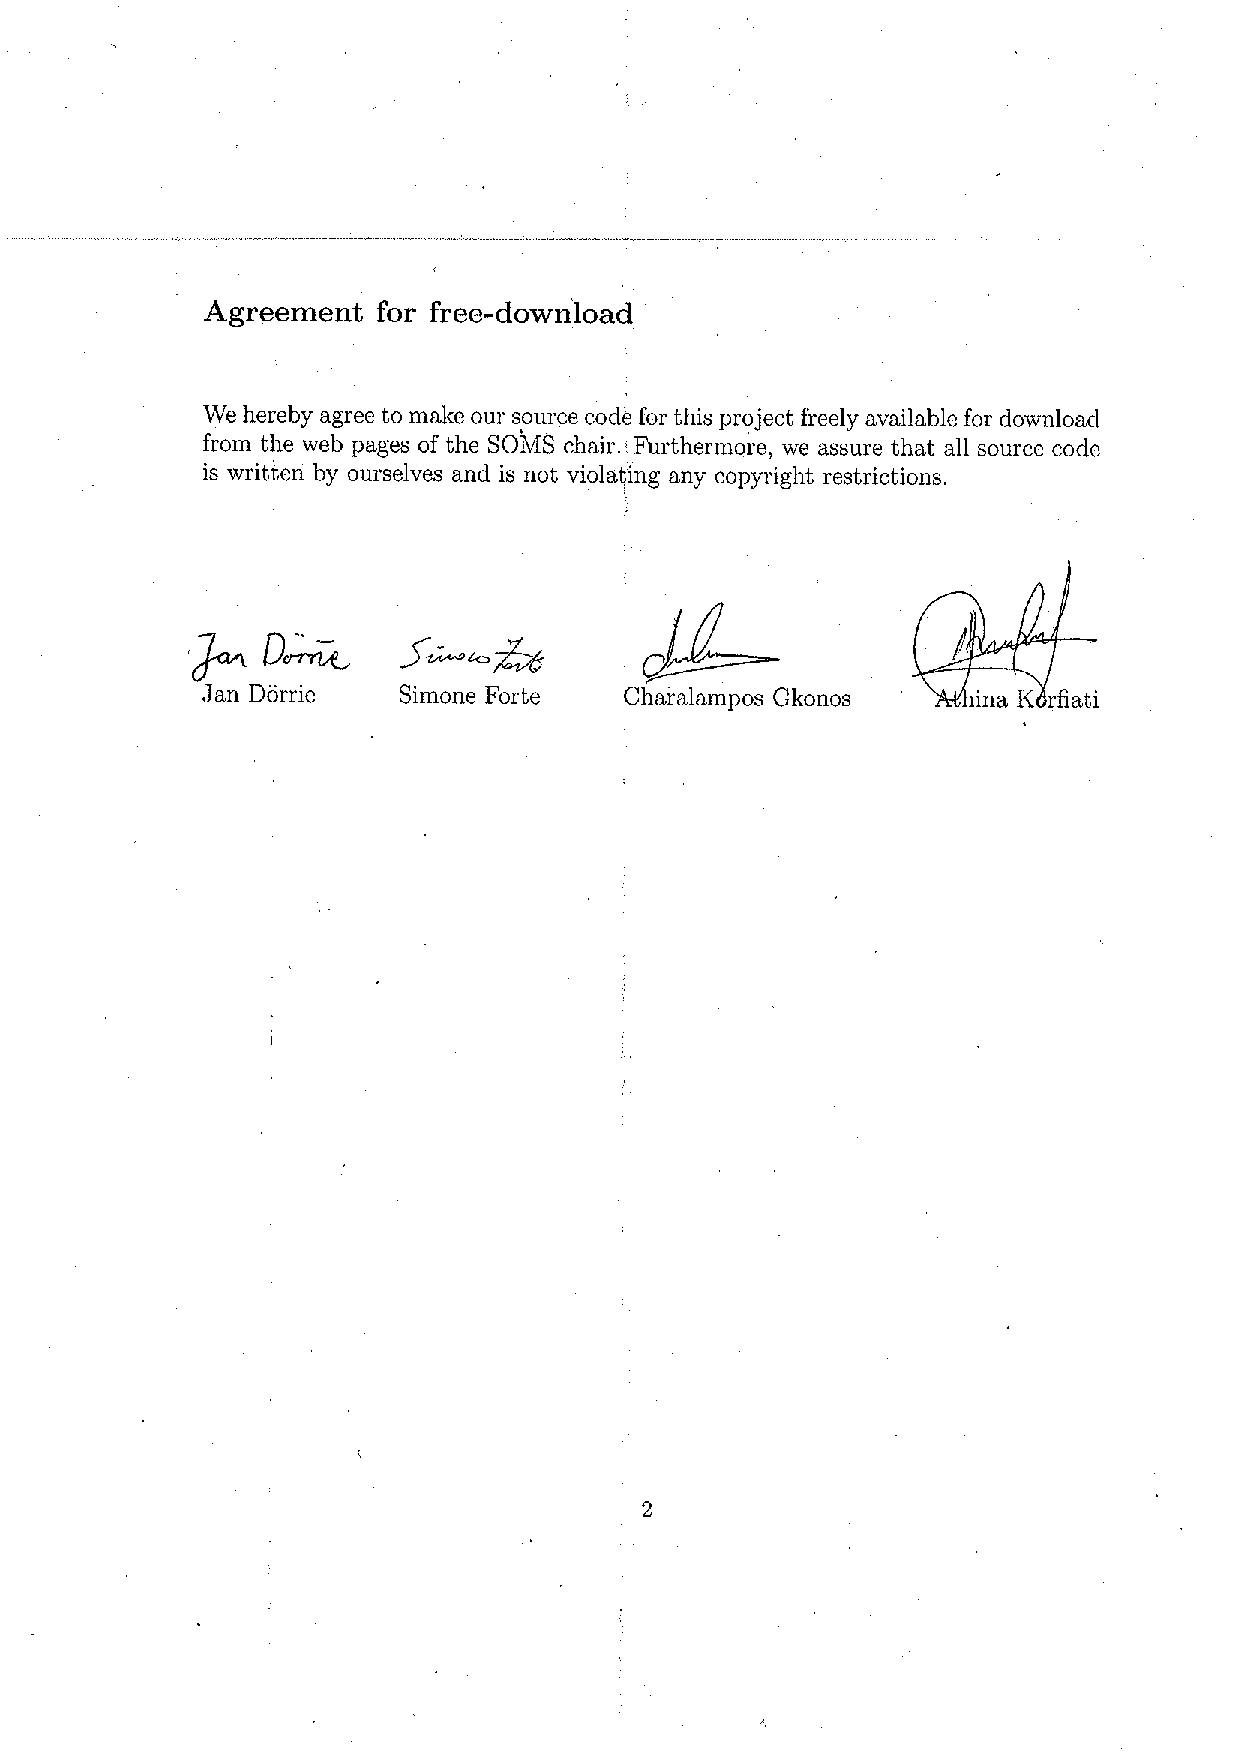
\includepdf[pages={1}]{../Agreement_for_free-download.pdf}

\newpage

%%%%%%%%%%%%%%%%%%%%%%%%%%%%%%%%%%%%%%%



% IMPORTANT
% you MUST include the ETH declaration of originality here; it is available for download on the course website or at http://www.ethz.ch/faculty/exams/plagiarism/index_EN; it can be printed as pdf and should be filled out in handwriting

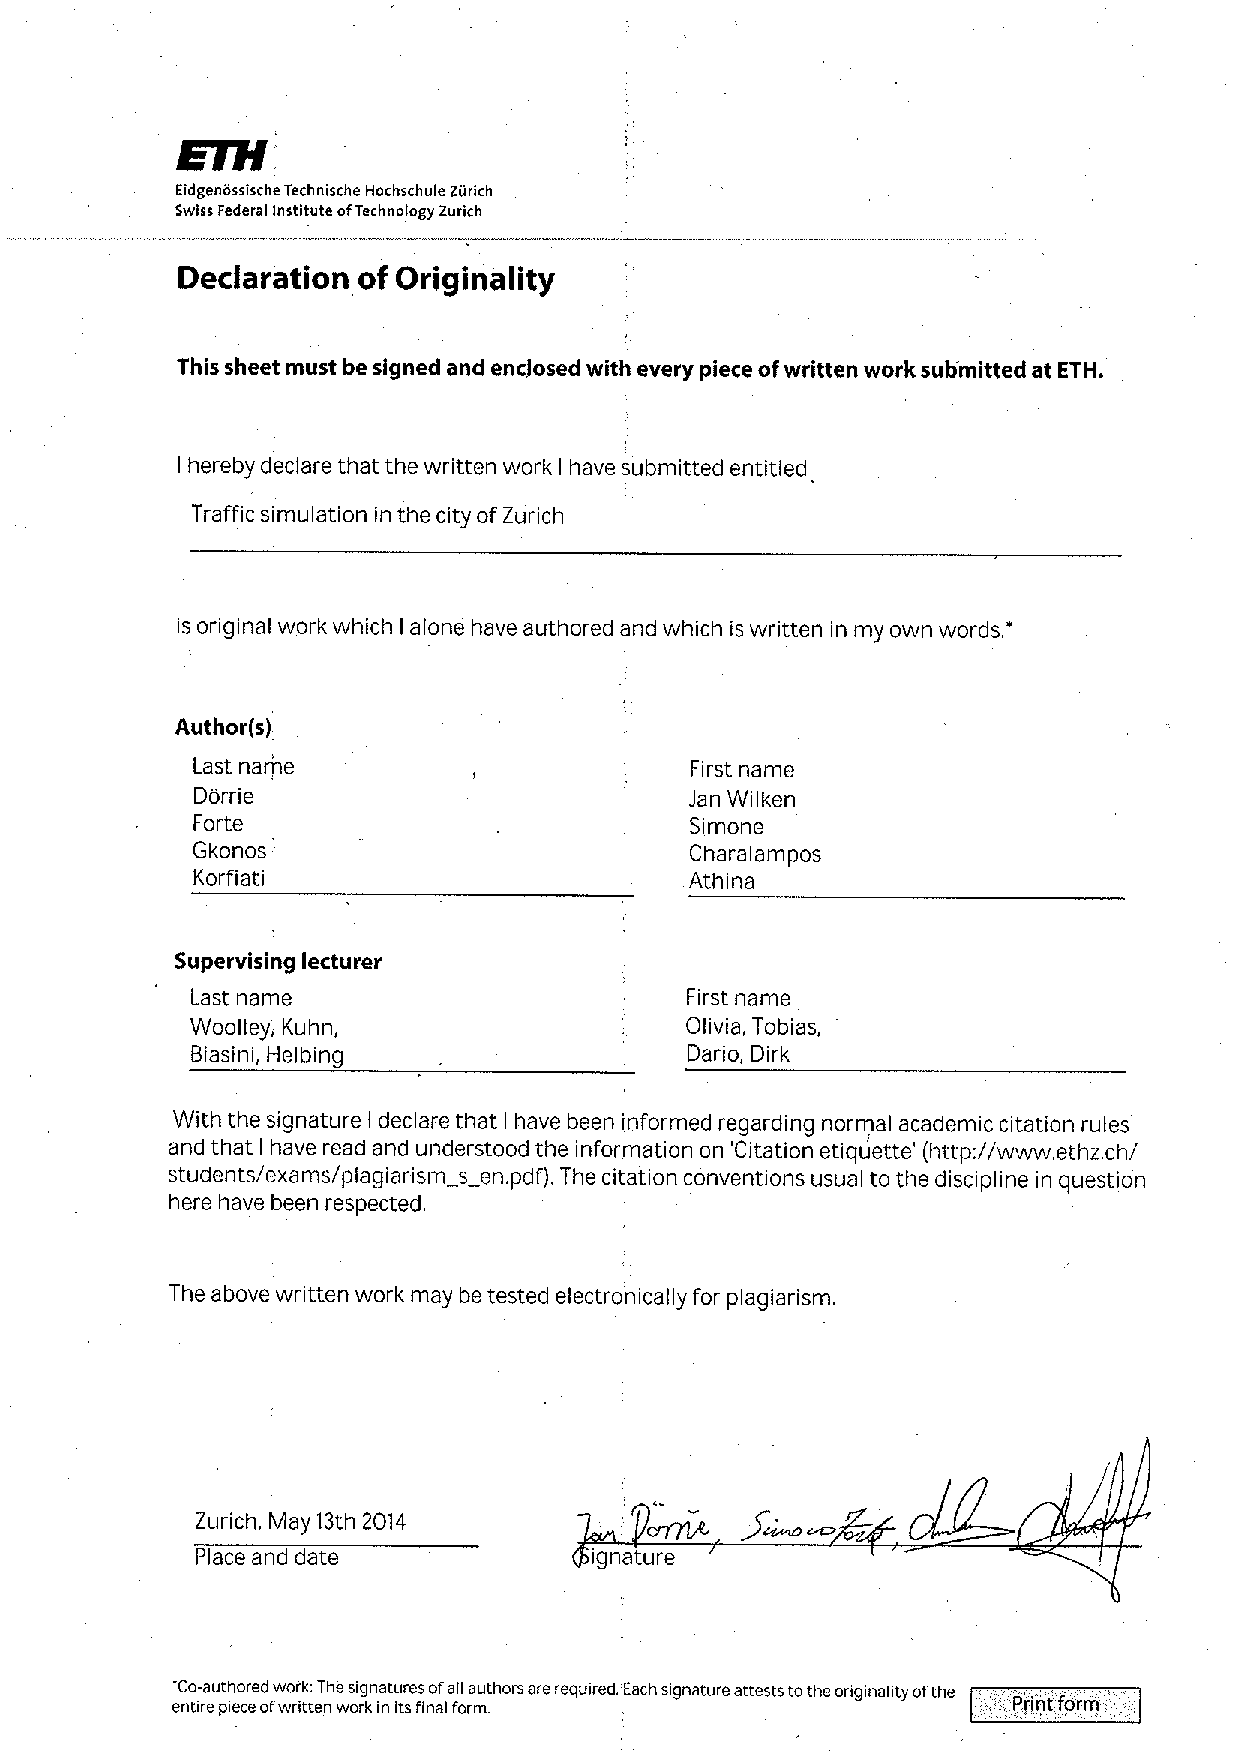
\includepdf[pages={1}]{../Declaration_of_Originiality.pdf}

%%%%%%%%%% Table of content %%%%%%%%%%%%%%%%%

\tableofcontents

\newpage

%%%%%%%%%%%%%%%%%%%%%%%%%%%%%%%%%%%%%%%



\section{Abstract}
In this paper, a traffic simulation for the city of Z\"urich is developed. The representation of traffic flows is a very useful tool for urban planning and is essential in cases that large scale construction works are planned. In the case of the city of Z\"urich, we were inspired from a proposed project for the construction of an underground tunnel that would connect the East and West side of the lake. The goal of this paper is to examine and derive conclusions whether such a tunnel would affect (improve or worsen) the traffic problem of the city center. More specifically, the traveling times from certain starting points to ending ones will be examined before and after the construction of such a technical work. At the end of the simulation, the results will be analyzed.

As an initial step, the route of every car is computed, using the shortest path algorithm (A* search algorithm), in the reduced road network that is selected for the project. Then, in order to model traffic propagation on given road segments, Cellular Automaton model is used. Finally, the planned tunnel will be introduced not in one, but more possible solutions, and its impact on the traffic situation for each one of them will be examined.


\section{Individual contributions}
In our project, all four team members were active and contributed in the development of the simulation. More specifically, MATLAB coding and implementation was done by Jan D\"orrie and Simone Forte. Charalampos Gkonos and Athina Korfiati were responsible for the data acquisition and data editing. The final analysis of the results, as well as the report preparation was performed by the whole team.

\section{Introduction and Motivations}
Traffic is a serious problem. Almost every big city in the world, no matter if it is in a developed or a developing country has to face this problem. Even in Z\"urich, the biggest city in Switzerland, where a very good system of public transportation exists and serves every corner of the city, the problem of traffic is not completely solved. Sometimes there is a need to look for innovative thoughts that may lead to perfect solutions. But first of all it is obvious that you have to evaluate all these alternatives in order to take the right decision. In this particular case study, a Highway Tunnel, proposed by the ARGE Z\"uriring consortium (G\"uller G\"uller architecture urbanism, Synergo, Heierli Engineering AG, Roland M\"uller, Metron AG, Ecoplan) to the Department of Civil Engineering of the Canton of Z\"urich in 2002 is examined. According to this ``Highway Tunnel Z\"urich'' project, a tunnel that connects the two sides of the Lake of Z\"urich is proposed among some other alternatives. (G\"uller G\"uller architecture urbanism, 2001-2002)

\begin{figure}[ht]
	\begin{center}
		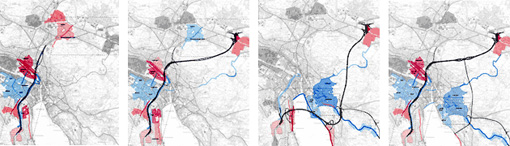
\includegraphics[width=\linewidth]{../img/GG03_1a.jpg}
	\end{center}
	\caption{The four different solutions proposed in ``Highway Tunnel Z\"{u}rich'' project \cite{GGau}}
	\label{fig:tunnel}
\end{figure}

With the present case study the goal is to develop an appropriate and efficient traffic model based on the available public data. This model can be used to visualize the existing traffic situation in the city of Z\"urich, as well as to describe the expected results after the construction of the tunnel. Based on this knowledge, it is possible to draw useful conclusions, which can be analyzed in order to evaluate the impact of such a tunnel. As far as it concerns the expected results, it is not easy to make a prediction. The problem is that the construction of huge technical works has always many more impacts in an area than the obvious (i.e. possible rise of the population living near the tunnel exits). An in-depth study is always needed which takes into account both qualitative and quantitative factors like potential future development opportunities, construction cost, maintenance and safety and many more. Nevertheless, for the purpose of the present case study there was no need for a so detailed analysis and for that reason there is a higher probability of misjudgment.


\section{Description of the Model}
A classical urban transportation planning system model usually follows four steps:

\begin{itemize}
	\item \textbf{Trip generation} determines the frequency of origins or destinations of trips in each zone by trip purpose, as a function of land uses and household demographics, and other socio-economic factors.

	\item \textbf{Trip distribution} matches origins with destinations, often using a gravity model function, equivalent to an entropy maximizing model. Older models include the fratar model.

	\item \textbf{Mode choice} computes the proportion of trips between each origin and destination that use a particular transportation mode. (This modal model may be of the logit form, developed by Nobel Prize winner Daniel McFadden.)

	\item \textbf{Route assignment} allocates trips between an origin and destination by a particular mode to a route. Often (for highway route assignment) Wardrop's principle of user equilibrium is applied (equivalent to a Nash equilibrium), wherein each driver (or group) chooses the shortest (travel time) path, subject to every other driver doing the same. The difficulty is that travel times are a function of demand, while demand is a function of travel time, the so-called bi-level problem. Another approach is to use the Stackelberg competition model, where users (``followers'') respond to the actions of a ``leader'', in this case for example a traffic manager. This leader anticipates on the response of the followers.”  (Wikipedia, n.d.)
\end{itemize}

The model we developed is loosely based on cellular automata. Every car is thus represented as an automaton which acts according to a very simple update rule; all the transitions will happen on a graph which represents the road network of a city, in this particular case this will be the city of Z\"urich. The model has two main parts:
\begin{itemize}
\item \textbf{Journey generation}: for every automaton we will generate a path that it will follow; this route will be fixed at the beginning and it will stay unchanged for the rest of the simulation. The way this routes will be generated will be based on a probability distribution defined by the CSVs files population.csv and companies.csv; what we aimed at modeling was the everyday morning journey of people from their houses to the workplace; we will thus have that the sources of the paths will be generated with a probability proportional to the number of people living in a certain area of the city and the destinations will be generated with a probability proportional to the number of companies situated in a certain area. Additionally to the city of Z\"urich we also took into account the population living in smaller towns south of the river which we aggregated as incoming and outgoing from the major highways located in the south of Z\"urich; this has been necessary in order to evaluate the impact of a tunnel in that area.
A visualization of this can be seen in figure \ref{fig:pop_data}.

\begin{figure}[tbh]
	\begin{center}
		\includegraphics[width=\linewidth]{../img/population_distribution.png}
	\end{center}
	\caption{Visualization of the chosen population and company hubs. Red dots how population areas and yellow dots company ares.}
	\label{fig:pop_data}
\end{figure}

\item \textbf{Route planning}:  After the intended journey for an automaton has been generated we will generate the actual path that the automaton intends to follow. We have in particular considered a realistic assumption that the paths will be decided at the beginning of the journey to be the shortest path between two locations and will remain unchanged regardless of the traffic situation of a road.
\item \textbf{Journey execution}: At this point the automaton knows the actual path it wants to follow. It will thus be initialized in its starting location and at every time step, having length in milliseconds equal to \textbf{m}, it will simply advance of a quantity equal to the minimum between the distance it can travel given that it travel for \textbf{m} milliseconds at the maximum speed allowed by the road it is following and the distance of the next car on the path minus a safety distance. To decide in which order update the cars in a timestep we will simply iterate on the cars in a random order and all the decisions for a car will be taken considering the position of the other cars at the time in which the car is updated.
\end{itemize}

\section{Implementation}
We started out by obtaining the OpenStreetMap file that contains Z\"urich.
In order to do so we downloaded a recent Switzerland extract from \emph{Geofabrik} \cite{geofab} and then extracted the boundaries of Z\"urich with the tool \emph{Osmconvert} \cite{osmconv}.
Afterwards we used another tool called \emph{Osmosis}\cite{oosmosis} to limit our data to the roads in Z\"urich.
Furthermore we modified the data using \emph{JOSM} which enabled us to simplify the road network, making our algorithms more efficient.
Once we removed small isolated connected components resulting from clipping the data to Z\"urich with self-written Python scripts
we extracted a simple graph structure, just containing a list of nodes and edges.
Each node was annotated with its id, as well as latitude and longitude.
For each edge we referenced existing nodes by their id and added the allowed maximum speed on this edge.
This data we also extracted with the help of Python scripts and interpolated from similar results in case this data was missing.
Afterwards we wrote an A-Star algorithm implementation in C++ in order to find the shortest path between two given nodes in the graph.
Initially we had used Dijkstra's algorithm for this, however once we realized that this is a prime example for A Star using the Euclidean distance we switched and obtained a much faster algorithm.
We considered implementing this algorithm directly in MATLAB, however the inconvenience of working with adjacency lists and the overall much slower performance forced us to write a C++ implementation.
However, by turning it into a mex file, we were still able to call this function directly from our MATLAB code, hence the integration was very smooth.
We further wrote a wrapper around this function in MATLAB, that would perform sanity checks on the input and exit gracefully in case there is an error.

The MATLAB implementation mostly consists of two parts, an initialization part and an update part. In the initialization the main data structures and parameters of the model are set up; we thus generate the routes for every car, picking starting and ending location according to a probability distribution specified by the CSVs files (reference...) and the actual path will be generated by computing the shortest path between the two locations. In the update part, for every timestep, we compute the new locations of every car according to the way specified earlier in the Description of the Model section and we compute the new GEO coordinates of the cars which are then given back to the Javascript client.

Finally we made use of the Javascript Library \emph{Leaflet}\cite{leaflet} to visualize our results on the actual map of Z\"urich.
We enabled communication between MATLAB and Javascript using the included Java classes for socket communication.
The Javascript code issues HTTP GET requests telling the MATLAB implementation which methods to perform.
The actions include initializing and advancing the simulation.
After each simulation step we passed the current car locations as a JSON object through the socket.
For encoding the object as a JSON string we made use of Google's Gson library\cite{gson}.
The Javascript implementation then made sure to display the cars at the right locations on the map.
\section{Simulation Results and Discussion}
\subsection{In correlation with the number of cars}
The figure that is presented below, shows that there is a strong correlation between the travelling time and the number of cars that use the road network. Of course this is something that is expected mainly because of the limitations of the existing road network (there is no projection for a huge number of cars in the city of Z\"urich). More specifically there is an average increase of around 25\% to the travelling time when the number of cars is going from 400 to 1600, more than 50\% when the number of cars changes from 2000 to 4000, and finally a massive 100\% when the number of cars increases from 400 to 4000.

\begin{figure}[tb]
	\begin{center}
		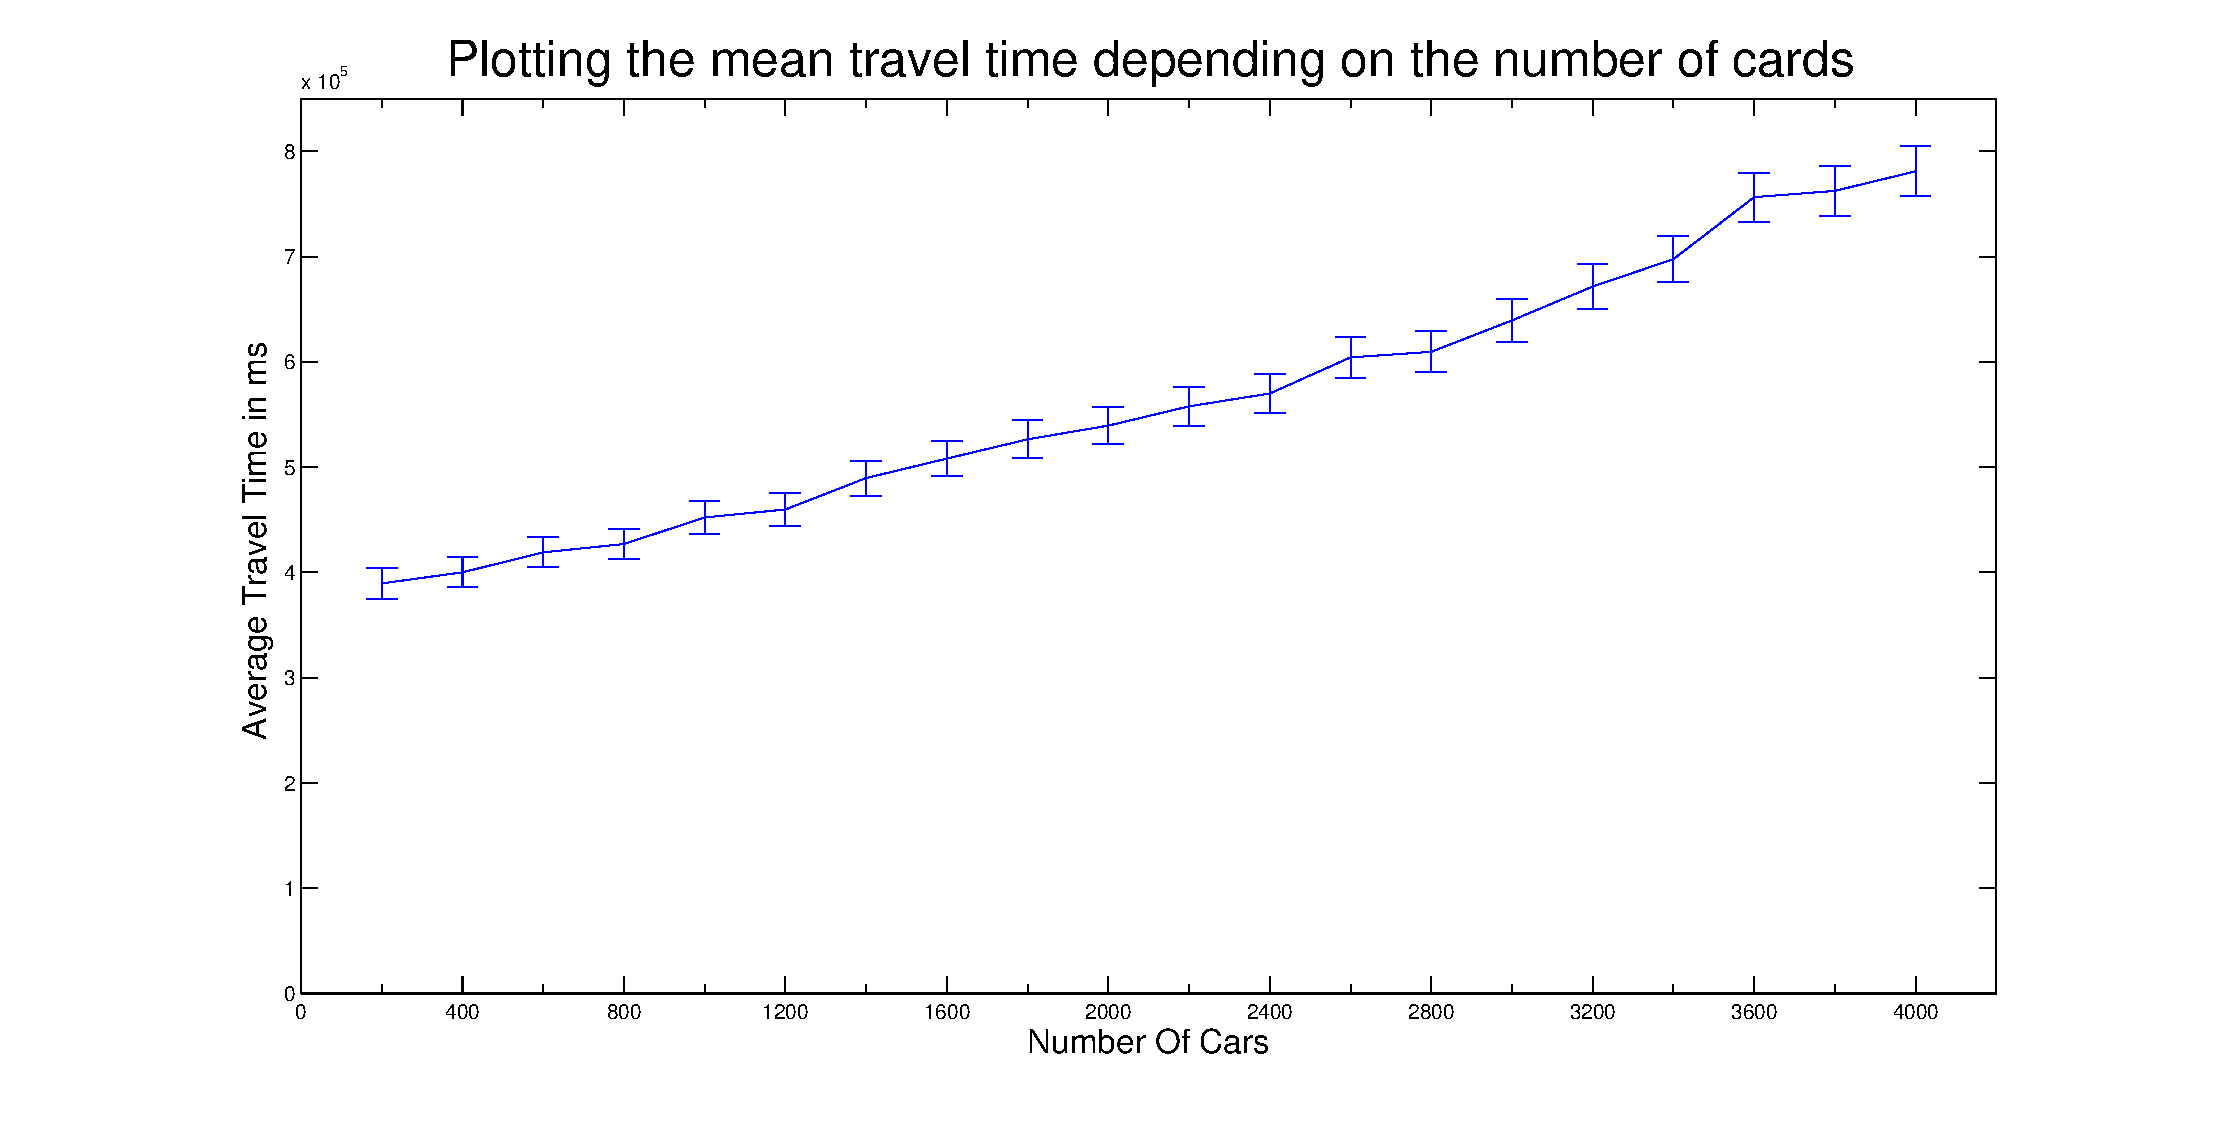
\includegraphics[width=\linewidth]{Travel_Times.eps}
	\end{center}
	\caption{Plot of travel times with regard to increasing number of cars on the road}
	\label{fig:figure1}
\end{figure}

\subsection{In correlation with the chosen position for the tunnel construction}
From the sixteen different scenarios that are evaluated it comes out as a conclusion that with the available data, the alternative positions for the tunnel construction do not influence that much the average time that a driver needs to move from his starting point to his destination. This probably happens because all these sixteen alternatives are close enough as it can be seen in Figure \ref{fig:tunnel_pos}.

\begin{figure}[htb]
	\begin{center}
		\includegraphics[width=\linewidth]{../img/tunnel_positions.png}
	\end{center}
	\caption{Visualization of the various start and end points of the tunnel.
	Red dots show possible starting positions and yellow dots possible end positions.}
	\label{fig:tunnel_pos}
\end{figure}

\subsection{In correlation with the construction of the tunnel in general} % (fold)
\label{sub:in_correlation_with_the_construction_of_the_tunnel_in_general}
In the last simulation the average travelling time for the drivers before and after the construction of the tunnel is evaluated. The simulation results are summarized in table \ref{tab:times}.


\begin{table}[tb]
	\caption{Average travel time in milliseconds with regard to tunnel location and number of cars}
	\label{tab:times}
	\begin{center}
		\begin{tabular}{rrccc}
		\toprule
		start node id & end node id & 500 cars & 1000 cars & 2000 cars \\
		\midrule
			170424926 & 1199905289 & 398570 & 447040 & 576070 \\
			170424926 & 2114250 & 419070 & 444740 & 542180 \\
			170424926 & 2114253 & 410970 & 453580 & 564700 \\
			170424926 & 80041651 & 404440 & 441430 & 541860 \\
			170425961 & 1199905289 & 420470 & 453320 & 544150 \\
			170425961 & 2114250 & 423860 & 443500 & 533280 \\
			170425961 & 2114253 & 421850 & 435940 & 539880 \\
			170425961 & 80041651 & 399220 & 450070 & 555110 \\
			28961405 & 1199905289 & 409720 & 441690 & 527970 \\
			28961405 & 2114250 & 414000 & 447560 & 520660 \\
			28961405 & 2114253 & 393170 & 447390 & 536280 \\
			28961405 & 80041651 & 401790 & 443810 & 553050 \\
			329026137 & 1199905289 & 417620 & 440940 & 553870 \\
			329026137 & 2114250 & 424000 & 440600 & 533280 \\
			329026137 & 2114253 & 407270 & 439130 & 531330 \\
			329026137 & 80041651 & 412490 & 441830 & 536610 \\
			--- & --- & 400872 & 471644 & 545545 \\
		\bottomrule
		\end{tabular}
	\end{center}
\end{table}



From the examination and interpretation of this simulation results it is obvious that travel time is reduced in the case the tunnel is built. The whole traffic situation in the centre of the city is improved and there are less conjunction points compared to the initial situation. More specifically, it is underlined by the results that...

% subsection in_correlation_with_the_construction_of_the_tunnel_in_general (end)

\section{Summary and Outlook}
The present case study tries to visualize the traffic situation in the city of Z\"urich and evaluate the impact that a tunnel construction could have on the travel time, especially between the two sides of the lake. The research question defined in the beginning of the research was answered and the conclusion was that the tunnel could improve the travel time for the benefit of the drivers using the road network of Z\"urich. For the implementation of the simulation, many consumptions were made (e.g. for the population and the travelling purpose) and the data used were limited. For this reason, there are still enough points for improvement.

However, the simulation model is a good base for testing real and official data for the city of Z\"urich and this is yet a point for future exploration. Future work on this topic should include better data acquisition. The data should refer to a wider region and not focus specifically in the city of Z\"urich. The main reason for that is that such a technical work is usually expected to influence a wider area and a significantly larger amount of people.


% \section{References}

\newpage
\printbibliography


\section*{Appendix}

	\subsection*{C++ Code}
	\lstset{language=C++,
		basicstyle=\footnotesize,
		keywordstyle=\color{blue}\footnotesize,
		stringstyle=\color{red}\footnotesize,
		commentstyle=\color{ForestGreen}\footnotesize,
		morecomment=[l][\color{magenta}]{\#}
	}

	\subsubsection*{A Star C++ Implementation}
		\lstinputlisting{../../code/a_star_mx.cpp}

	\subsection*{MATLAB Code}
		\lstset{language=Matlab,%
	    %basicstyle=\color{red},
	    breaklines=true,%
	    morekeywords={matlab2tikz},
	    keywordstyle=\color{blue},%
	    morekeywords=[2]{1}, keywordstyle=[2]{\color{black}},
	    identifierstyle=\color{black},%
	    stringstyle=\color{red},
	    commentstyle=\color{ForestGreen},%
	    % showstringspaces=false,%without this there will be a symbol in the places where there is a space
	    % numbers=left,%
	    % numberstyle={\tiny \color{black}},% size of the numbers
	    % numbersep=9pt, % this defines how far the numbers are from the text
	    emph=[1]{for,end,break},emphstyle=[1]\color{blue}, %some words to emphasise
	    %emph=[2]{word1,word2}, emphstyle=[2]{style},
	}

		\subsubsection*{MATLAB Wrapper}
		\lstinputlisting{../../code/a_star.m}

\end{document}




